%%%%%%%%%%%%%%%%%%%%%%%%%%%%%%%%%%%%%%%%%
% baposter Portrait Poster
% LaTeX Template
% Version 1.0 (15/5/13)
%
% Created by:
% Brian Amberg (baposter@brian-amberg.de)
%
% This template has been downloaded from:
% http://www.LaTeXTemplates.com
%
% License:
% CC BY-NC-SA 3.0 (http://creativecommons.org/licenses/by-nc-sa/3.0/)
%
%%%%%%%%%%%%%%%%%%%%%%%%%%%%%%%%%%%%%%%%%

%----------------------------------------------------------------------------------------
%	PACKAGES AND OTHER DOCUMENT CONFIGURATIONS
%----------------------------------------------------------------------------------------

\documentclass[a0paper,portrait]{baposter}

\usepackage[font=small,labelfont=bf]{caption} % Required for specifying captions to tables and figures
\usepackage{booktabs} % Horizontal rules in tables
\usepackage{relsize} % Used for making text smaller in some places

\graphicspath{{figures/}} % Directory in which figures are stored

\definecolor{bordercol}{RGB}{40,40,40} % Border color of content boxes
\definecolor{headercol1}{RGB}{186,215,230} % Background color for the header in the content boxes (left side)
\definecolor{headercol2}{RGB}{80,80,80} % Background color for the header in the content boxes (right side)
\definecolor{headerfontcol}{RGB}{0,0,0} % Text color for the header text in the content boxes
\definecolor{boxcolor}{RGB}{186,215,230} % Background color for the content in the content boxes

\begin{document}

\background{ % Set the background to an image (background.pdf)
\begin{tikzpicture}[remember picture,overlay]
\draw (current page.north west)+(-2em,2em) node[anchor=north west]
{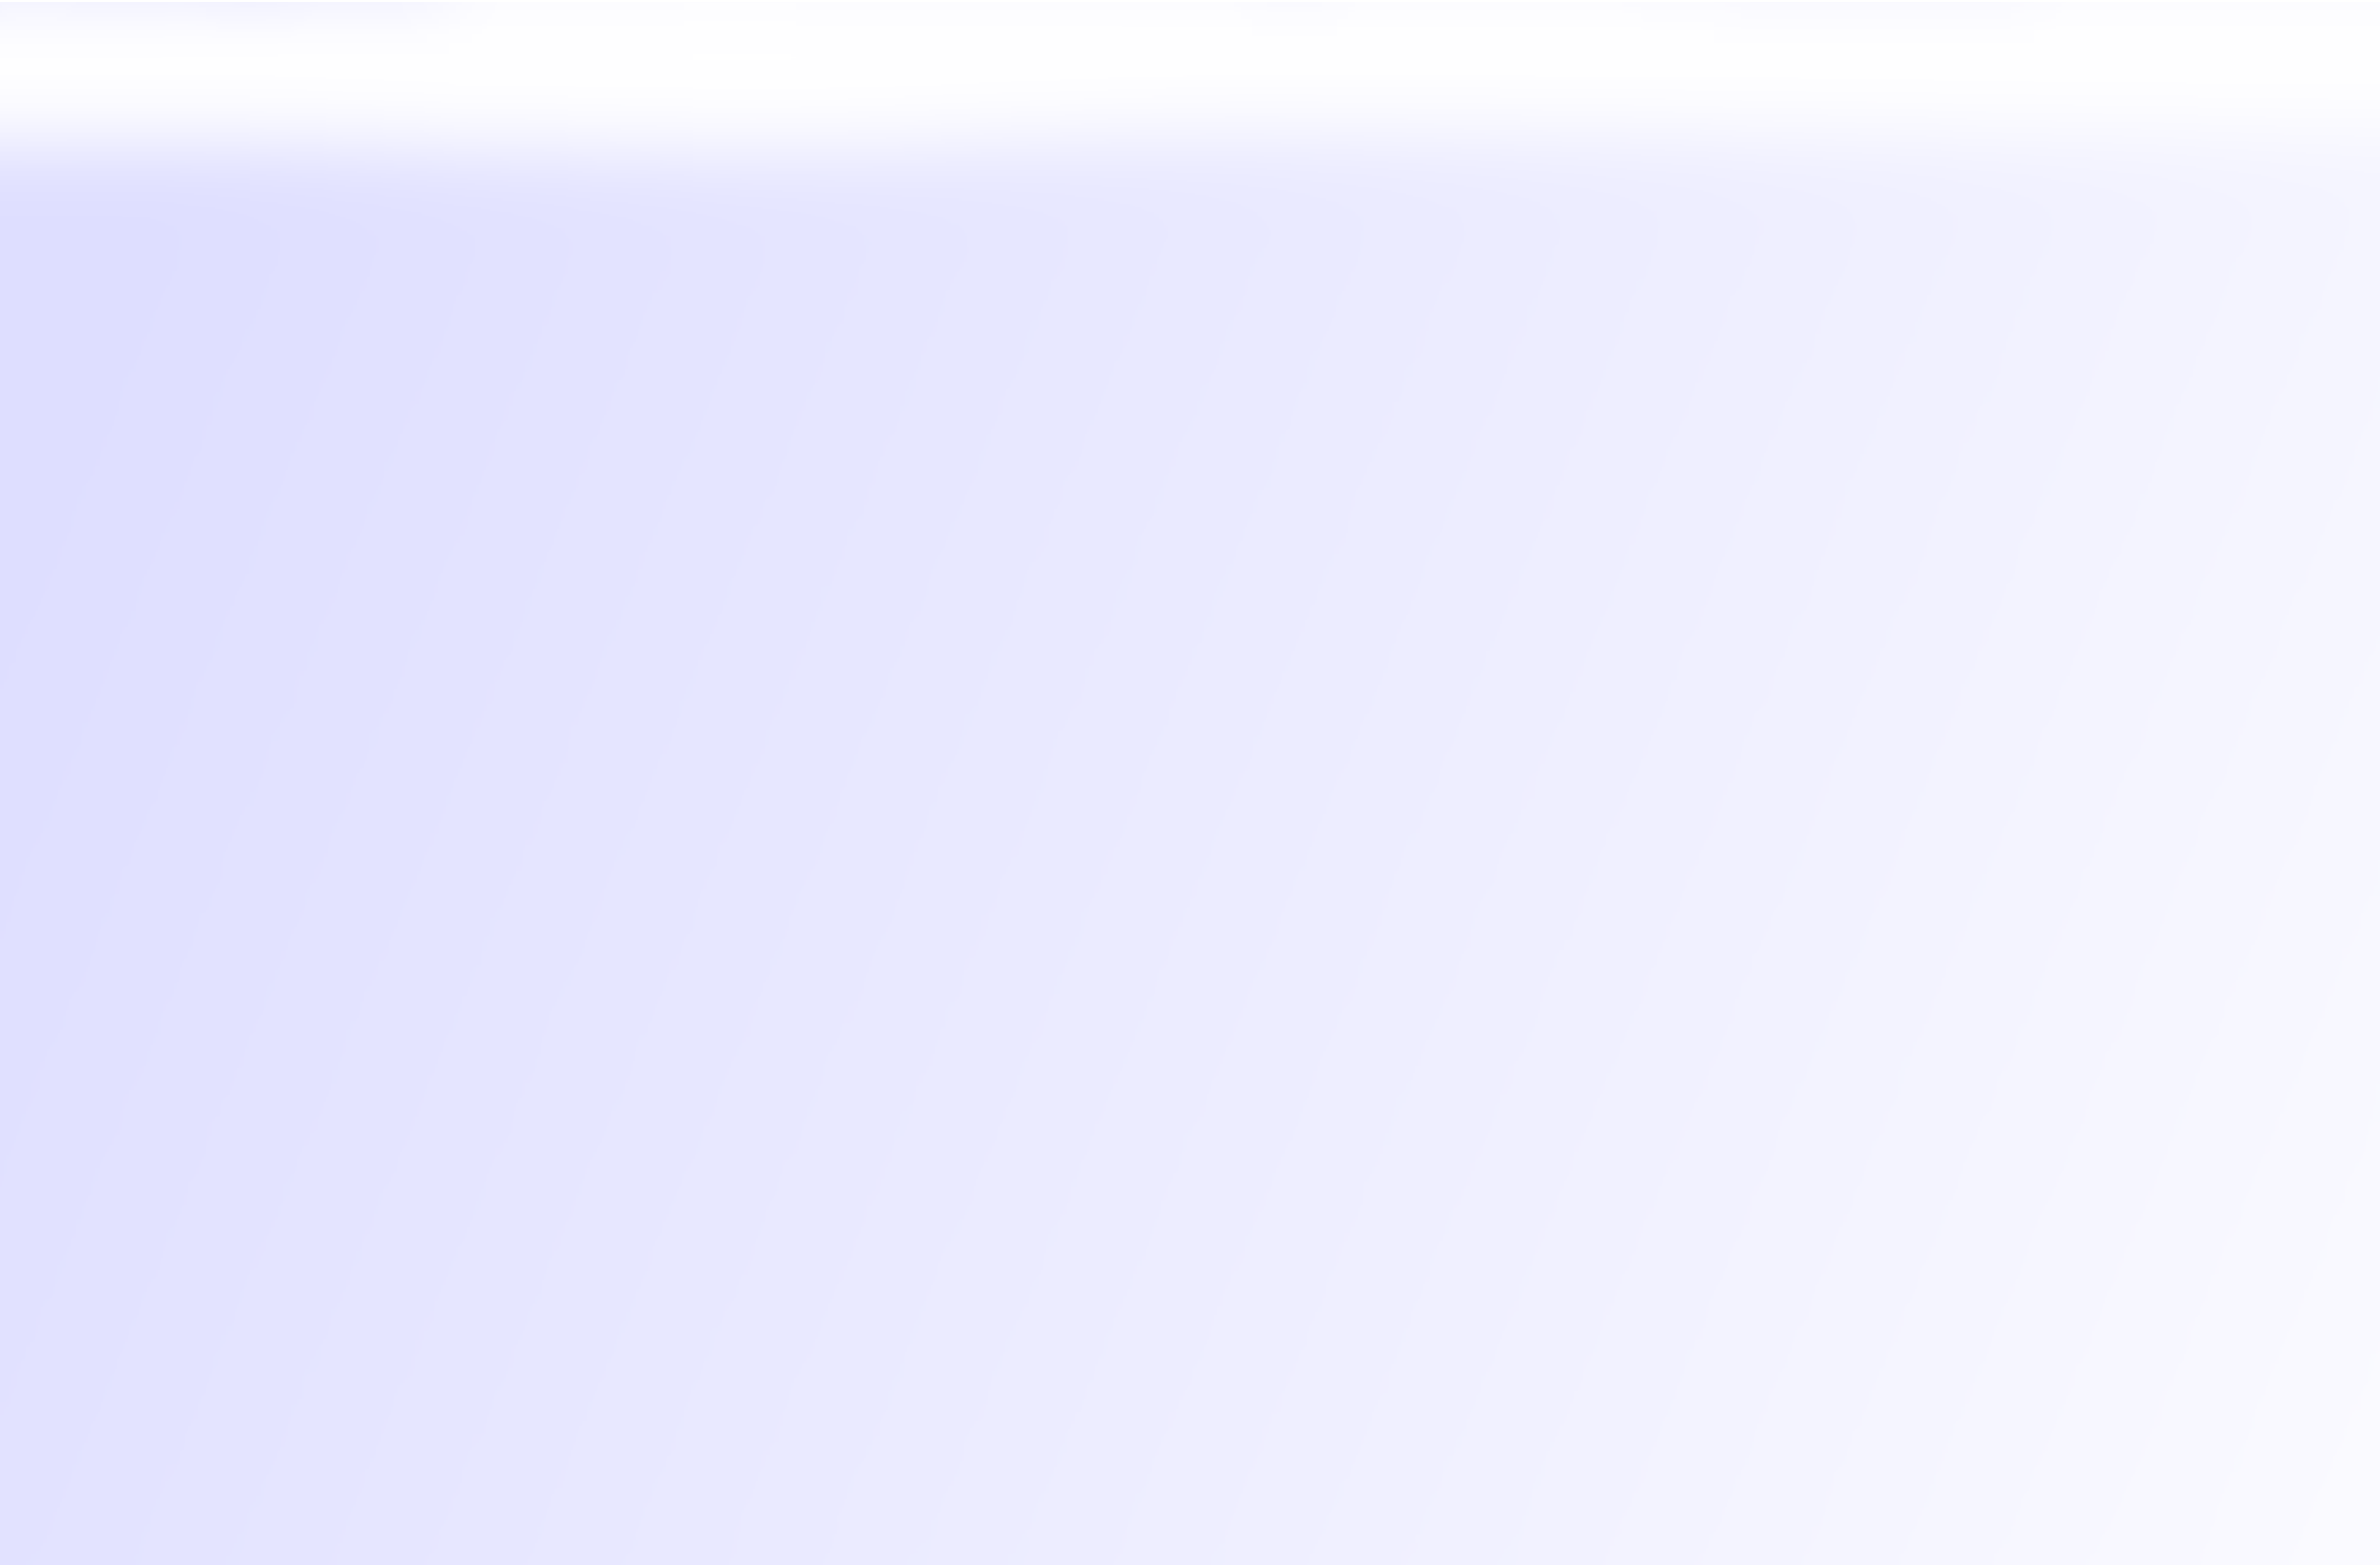
\includegraphics[height=1.1\textheight]{background}};
\end{tikzpicture}
}

\begin{poster}{
grid=false,
borderColor=bordercol, % Border color of content boxes
headerColorOne=headercol1, % Background color for the header in the content boxes (left side)
headerColorTwo=headercol2, % Background color for the header in the content boxes (right side)
headerFontColor=headerfontcol, % Text color for the header text in the content boxes
boxColorOne=boxcolor, % Background color for the content in the content boxes
headershape=roundedright, % Specify the rounded corner in the content box headers
headerfont=\Large\sf\bf, % Font modifiers for the text in the content box headers
textborder=rectangle,
background=user,
headerborder=open, % Change to closed for a line under the content box headers
boxshade=plain
}
{}
%
%----------------------------------------------------------------------------------------
%	TITLE AND AUTHOR NAME
%----------------------------------------------------------------------------------------
%
{\sf\bf Making games with Casanova} % Poster title
{\vspace{1em} Mohamed Abbadi, Francesco Di Giacomo, Agostino Cortesi, Pieter Spronck, Giulia Costantini, Giuseppe Maggiore\\ % Author names
{\smaller \{mohamed.abbadi, francesco.digiacomo, cortesi\}@unive.it, p.spronck@uvt.nl, costg@hr.nl, maggg@hr.nl}} % Author email addresses
{
\includegraphics[scale=0.15]{logo}} % University/lab logo

%----------------------------------------------------------------------------------------
%	INTRODUCTION
%----------------------------------------------------------------------------------------

\headerbox{Introduction}{name=introduction,column=0,row=0}{

Managing the flow of time and the coordination of multiple components in interactive applications (such as games) is a complex activity. For this reason, game development requires a lot of effort, even for (apparently) simple scenarios. We introduce a new language (Casanova 2), aimed at reducing cost and effort in the the development of interactive applications (through the use of specific constructs), while at the same time achieving high performance. The results obtained on a series of case studies are satisfactory with respect to this goal. 
}


%----------------------------------------------------------------------------------------
%	CONCLUSION
%----------------------------------------------------------------------------------------

\headerbox{Conclusion}{name=conclusion,column=0,below=introduction}{

Casanova 2 may offer a solution for the high development costs of games. The goal of Casanova 2 is to reduce the effort and complexities associated with building games. This is achieved through a language designed around games: Casanova 2 manages the game world through entities and rules, and offers constructs (wait and yield) to deal with the run-time dynamics. As shown by our results, we believe that we have taken a significant step towards reaching these goals. In fact, we achieved at the same time very good performance and ease of use, thereby empowering developers with limited resources.
}

%----------------------------------------------------------------------------------------
%	REFERENCES
%----------------------------------------------------------------------------------------

\headerbox{References}{name=references,column=0,below=conclusion}{

\smaller % Reduce the font size in this block
\renewcommand{\section}[2]{\vskip 0.05em} % Get rid of the default "References" section title
\nocite{*} % Insert publications even if they are not cited in the poster

\bibliographystyle{unsrt}
\bibliography{sample} % Use sample.bib as the bibliography file

}

%----------------------------------------------------------------------------------------
%	ACKNOWLEDGEMENTS
%----------------------------------------------------------------------------------------

\headerbox{Acknowledgements}{name=acknowledgements,column=0,below=references, above=bottom}{

\smaller % Reduce the font size in this block

We would like to thank Professors Aske Plaat, Fons Maes and Renzo Orsini for their support and contribution.
} 

%----------------------------------------------------------------------------------------
%	RESULTS 2
%----------------------------------------------------------------------------------------

\headerbox{Past}{name=past,span=2,column=1}{ % To reduce this block to 1 column width, remove 'span=2'

%------------------------------------------------

\begin{center}
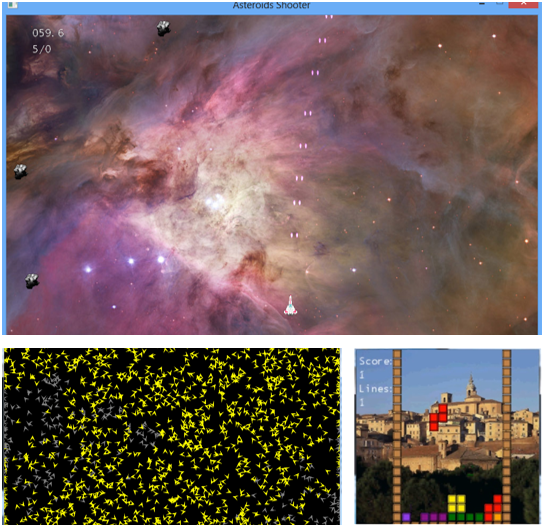
\includegraphics[width=0.3\linewidth]{cnv1Games}
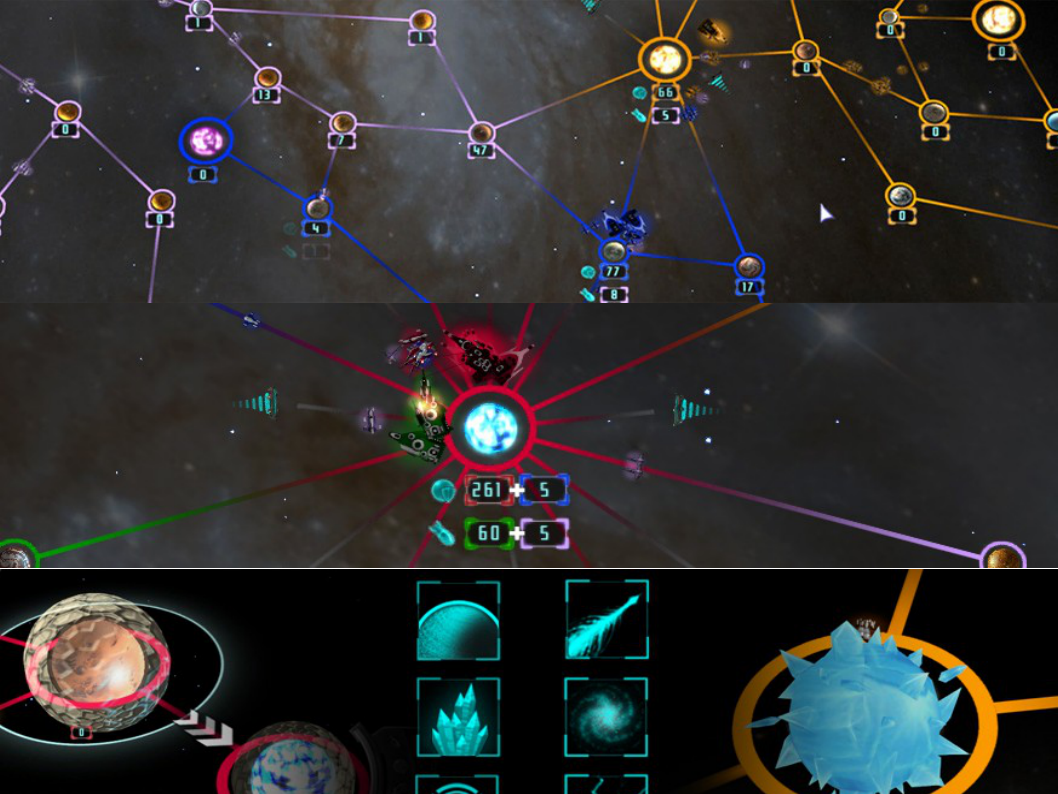
\includegraphics[width=0.30\linewidth]{galaxy_wars}
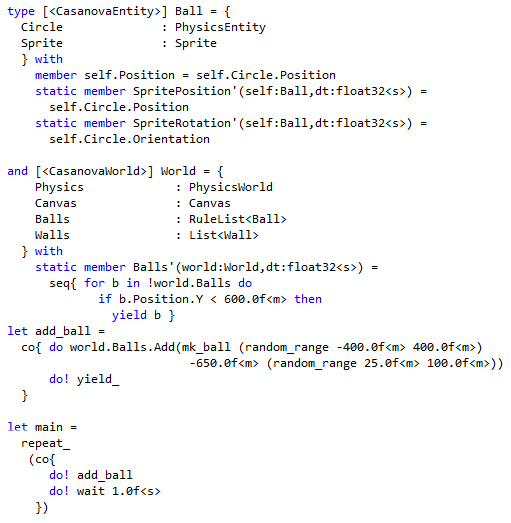
\includegraphics[width=0.3\linewidth]{fsharpCasanova}
\captionof{figure}{Some previous Casanova games (left); Galaxy Wars (right); Casanova implementation with F\# syntax}
\end{center}

}


\headerbox{Present}{name=present, below = past,span=2,column=1}{ % To reduce this block to 1 column width, remove 'span=2'

%------------------------------------------------

\begin{center}
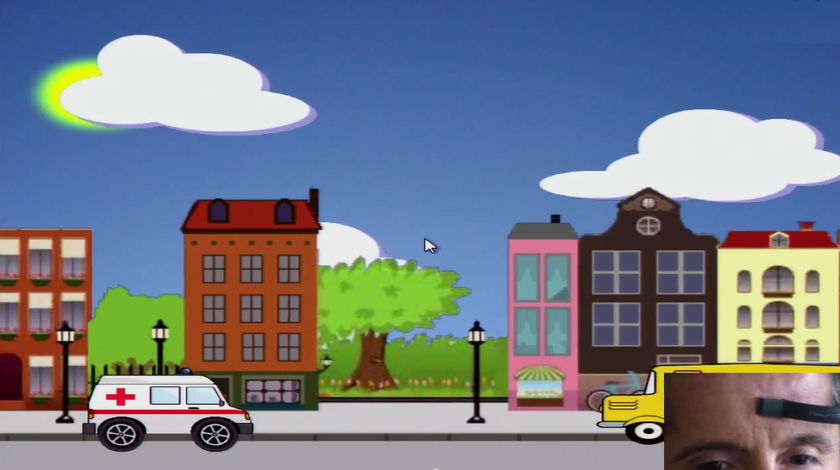
\includegraphics[width=0.30\linewidth]{ambulance}
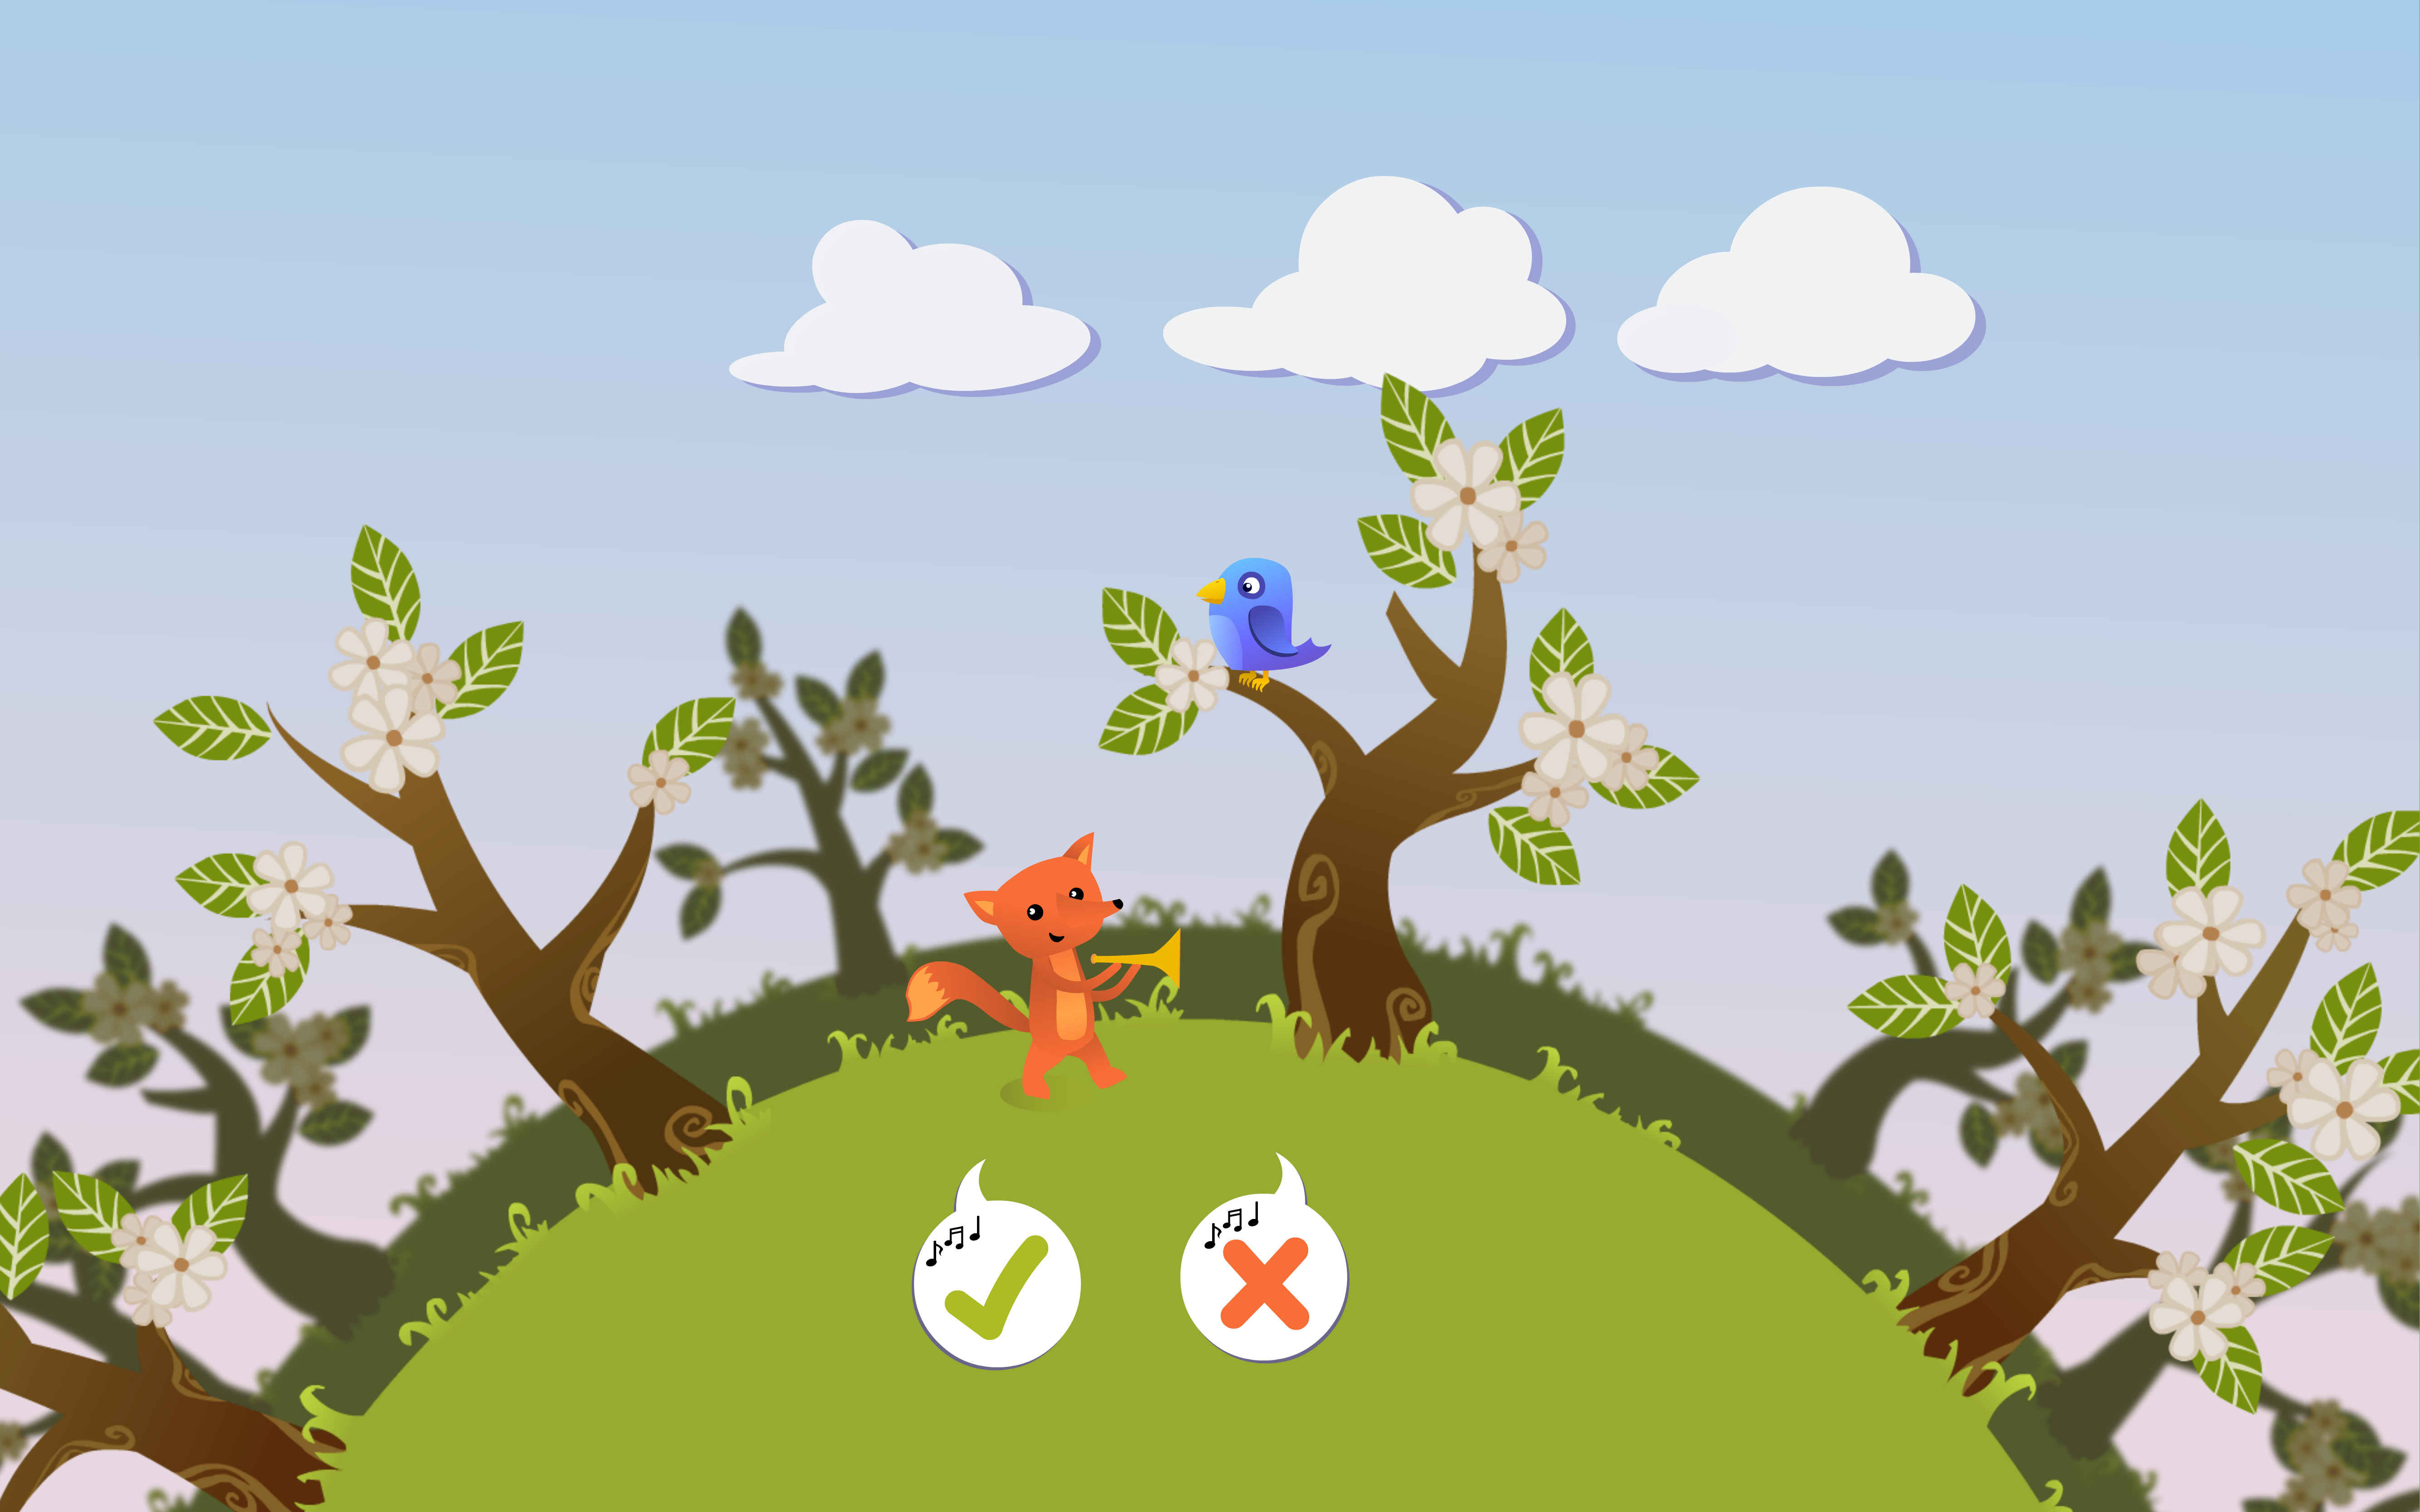
\includegraphics[width=0.30\linewidth]{dyslexia_game}
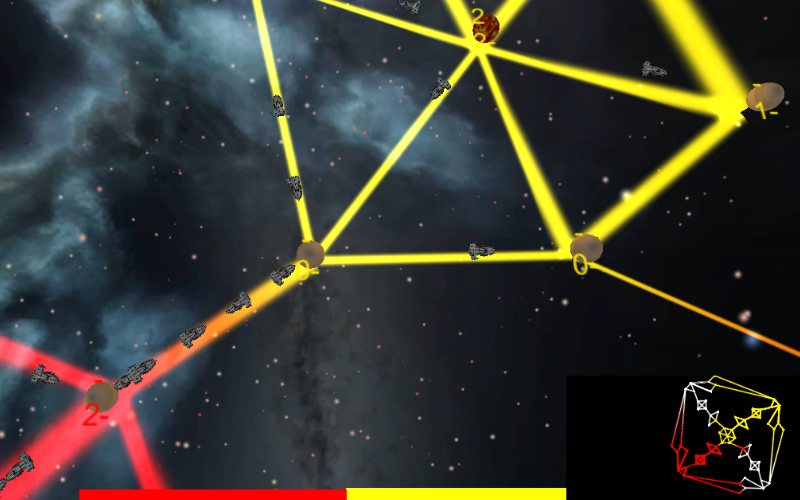
\includegraphics[width=0.30\linewidth]{rts}
\captionof{figure}{Ambulance game for pediatrics (left); Game for dyslexia detection (center); Real-time strategy game(right)}
\end{center}

\begin{center}
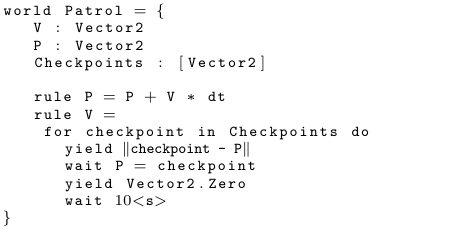
\includegraphics[width=0.4\linewidth]{cnv2Patrol}
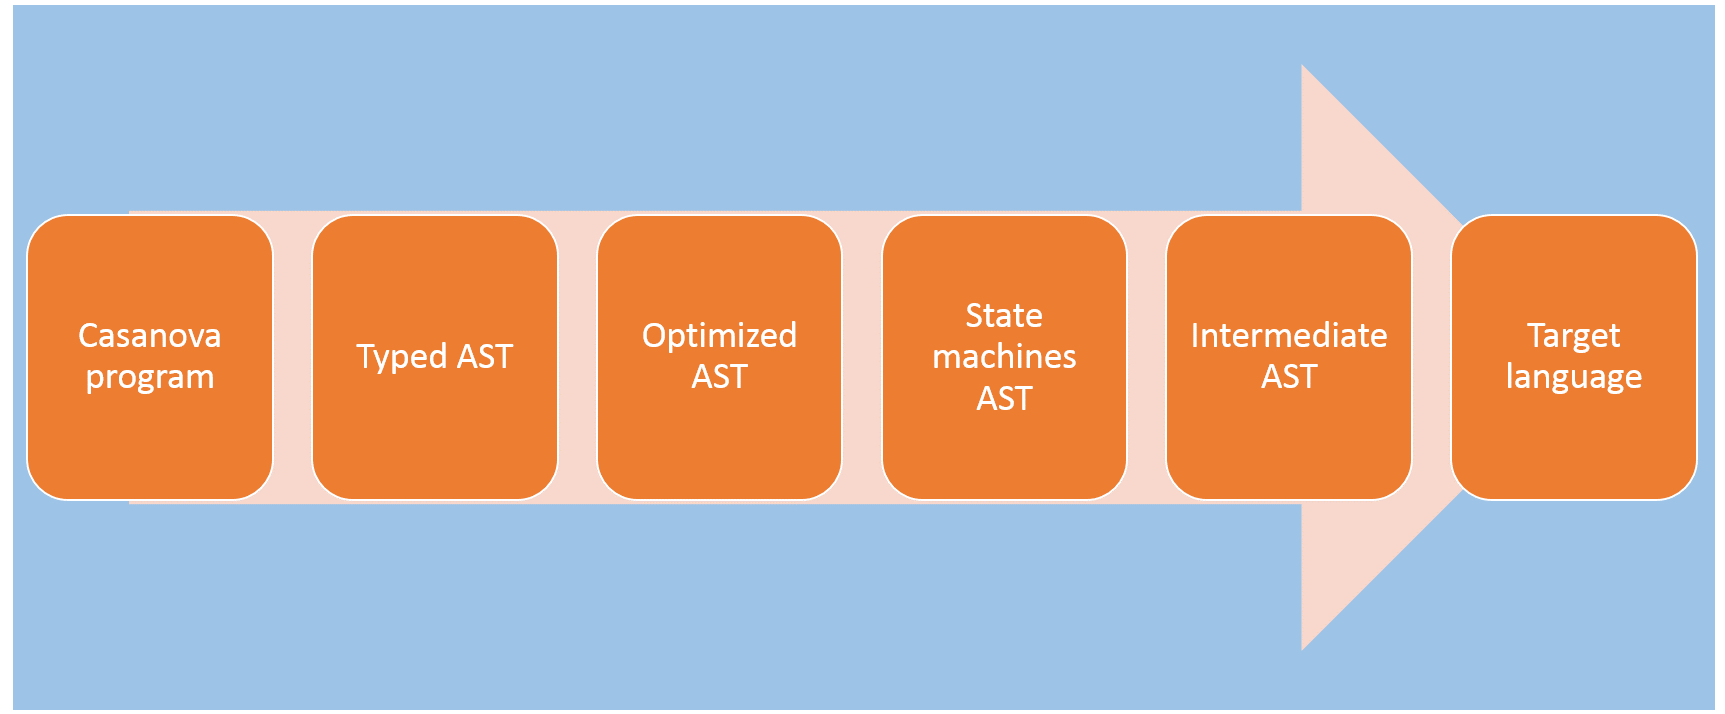
\includegraphics[width=0.5\linewidth]{casanovaLayerdCompiler}
\captionof{figure}{Casanova patrol sample (left); Casanova layered compiler (right)}
\end{center}

\begin{center}
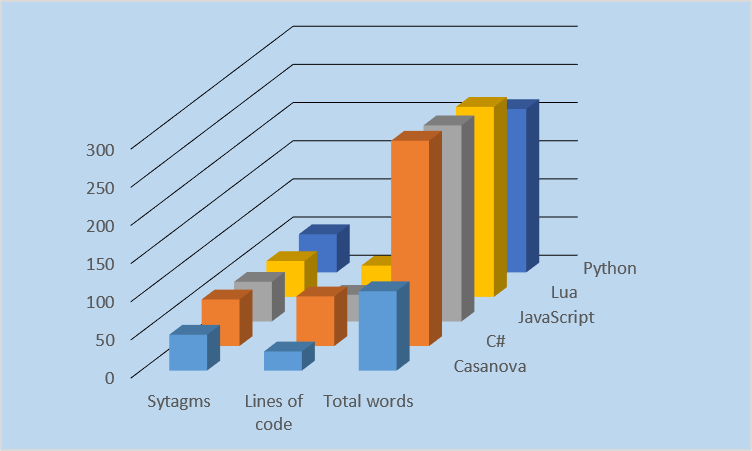
\includegraphics[width=0.3\linewidth]{syntax}
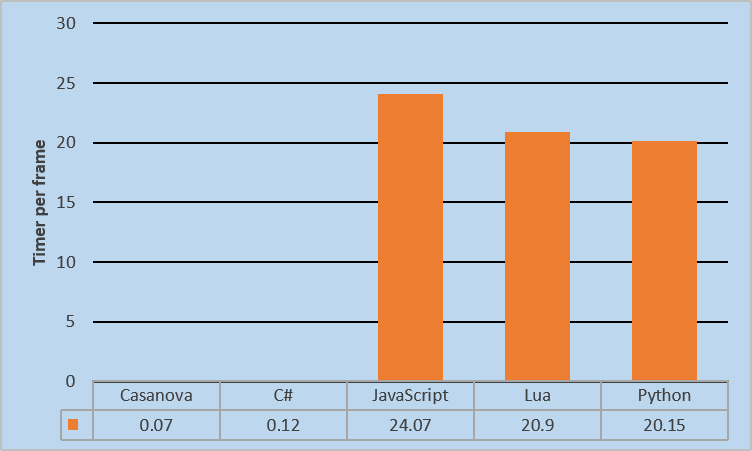
\includegraphics[width=0.3\linewidth]{performance}
\captionof{figure}{Casanova syntax evaluation (left); Casanova performance evaluation (right)}
\end{center}


}

\headerbox{Future - Casanova logic system}{name=future, below = present,span=2,column=1}{ % To reduce this block to 1 column width, remove 'span=2'

%------------------------------------------------

\begin{center}
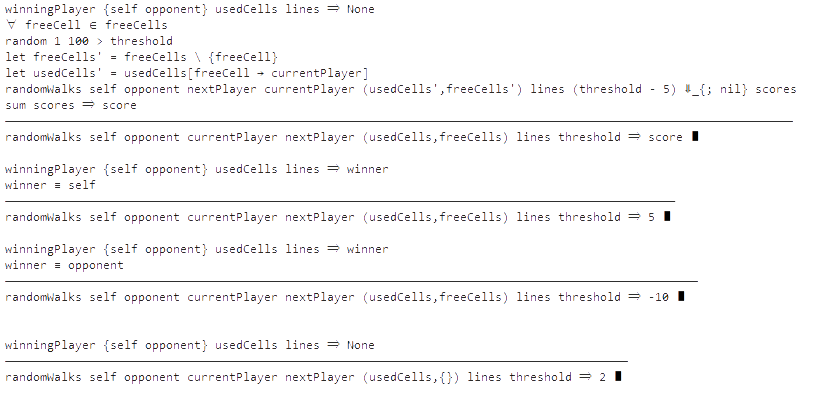
\includegraphics[width=0.6\linewidth]{random_walk}
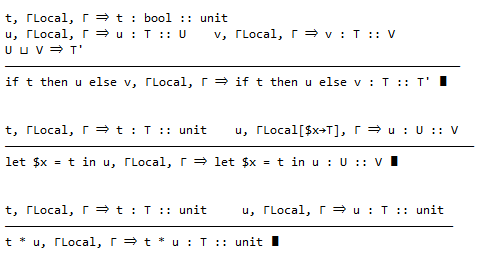
\includegraphics[width=0.4\linewidth]{typeSystem}
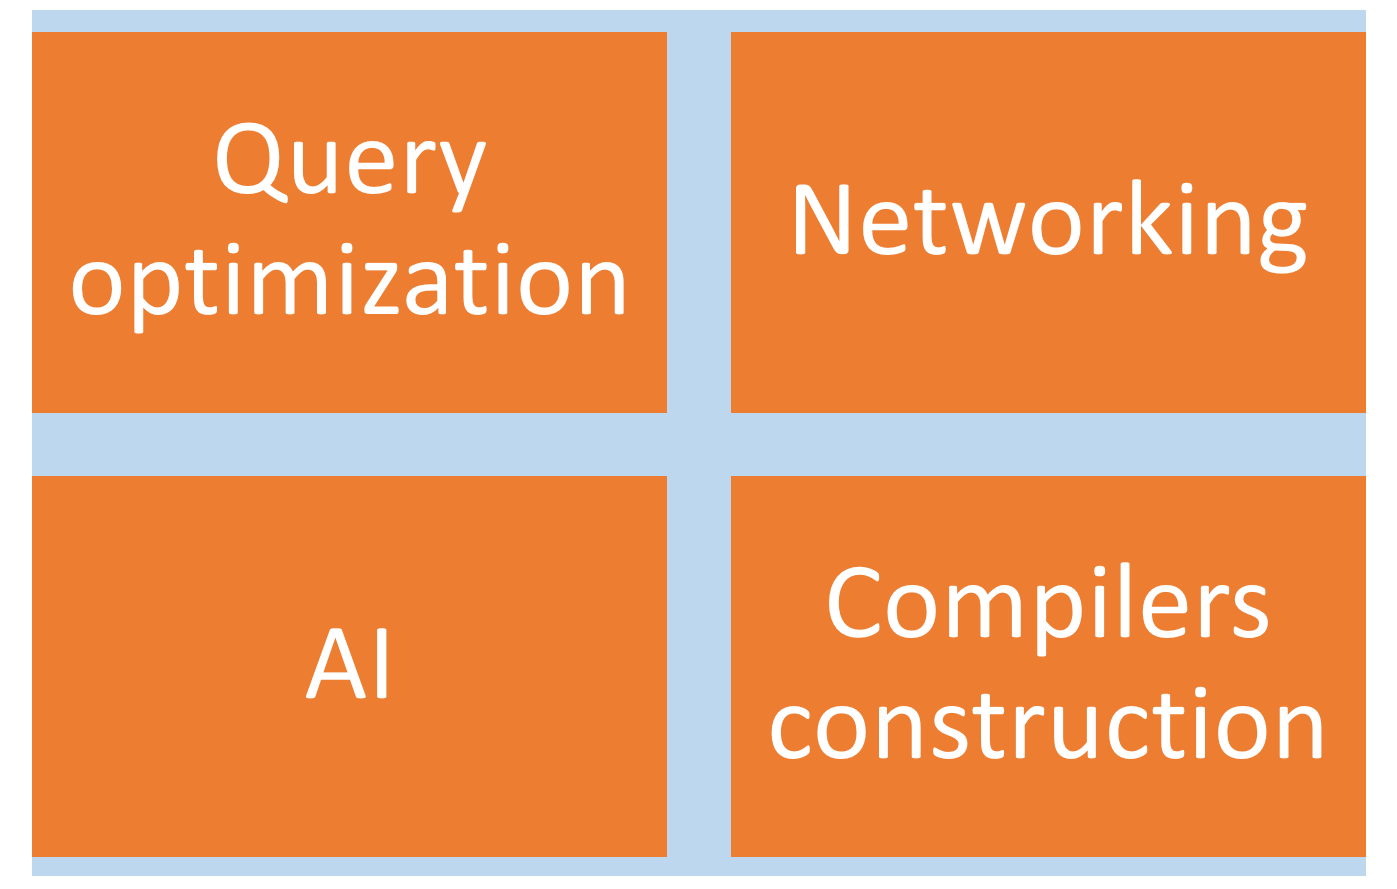
\includegraphics[width=0.35\linewidth]{future_applications}
\captionof{figure}{Random walk (left); Type checker (center); Future applications}
\end{center}

}

%----------------------------------------------------------------------------------------

\end{poster}

\end{document}